\documentclass[11pt]{article}
\usepackage[margin=1in]{geometry}
\usepackage{amsmath,amssymb,amsthm,booktabs,graphicx,hyperref,array,microtype,enumitem,longtable}
\newcommand{\Orbits}{840}
\newcommand{\NRules}{60}
\newcommand{\NStarts}{14}
\newcommand{\Cyc}{93}
\newcommand{\Esc}{405}
\newcommand{\Stuck}{342}
\newcommand{\Uncert}{0}
\newcommand{\ProvedCmp}{13626}
\newcommand{\NbCmp}{112}
\newcommand{\PrimRange}{2{,}000{,}000}
\newcommand{\NbrRange}{20{,}000}
\newcommand{\DegRange}{10^6}
\newcommand{\DescRange}{100{,}000}
\newcommand{\MaxSteps}{5}
\newcommand{\PrimeEnd}{14616}
\newcommand{\OtherEnd}{85384}
\newcommand{\FracMinAll}{0.136}
\newcommand{\FracMaxI}{0.154}
\newcommand{\MaxPrimes}{6}

\newtheorem{theorem}{Theorem}\newtheorem{proposition}[theorem]{Proposition}\newtheorem{lemma}[theorem]{Lemma}\newtheorem{corollary}[theorem]{Corollary}
\theoremstyle{remark}\newtheorem{remark}[theorem]{Remark}
\newcommand{\spf}{\operatorname{spf}}
\title{\textbf{UNNS-U2-RN}\\[2pt]\large Ranked-Neighbour Dynamics and Graph-Local Observability\\in the Reversible SELECT-II Graph}
\author{UNNS Research Collective}
\date{Version v001 \quad (separate addendum; UNNS-U2-TI v001 and UNNS-U2-TI-DYN v001 and all earlier releases are unchanged)}
\begin{document}\maketitle
\begin{abstract}\noindent
We ask what the arithmetic graph $G$ (edges $\{kN,k(N+1)^2\}$) exposes through its own local structure, with no sequence-specific controller. \textbf{RN-0} fixes a certification policy: a neighbourhood or degree is \emph{certified} only if every prime factor used is proved prime; runs lacking this are flagged. \textbf{RN-1} proves closed forms for seven ranked-neighbour operators and determines the full dynamics of six of them: the largest neighbour gives $x\mapsto(x+1)^2$; the second-largest is conjugate to it after one step; inverse-side and smallest-neighbour rules descend to squarefree numbers in at most $\log_4 x$ steps, and the smallest-neighbour rule then enters the 2-cycle $\{s,4s\}$. Forward moves never land on a prime, and a prime's only neighbours are $4p$ and $(p+1)^2$; hence every one of these rules visits at most one distinct prime. \textbf{RN-2} classifies \Orbits{} orbits of a registered 60-rule grammar: \Cyc{} cyclic, \Esc{} escaping, \Stuck{} stuck, none uncertified. Rules reading vertex degree reach up to \MaxPrimes{} distinct primes in finite orbits, with no theorem behind it. \textbf{RN-3} gives an observability ledger. Recognizing a prime vertex locally is a theorem; generating infinitely many primes by a graph-local rule is not shown, and the proved results are negative for the rank-based family.
\end{abstract}

\section{Scope and evidence levels}
Every statement carries one label. \textbf{Proved} (elementary argument in this note, no novelty claim). \textbf{Verified-bounded} (exact-integer check over a stated range; corroboration, not proof). \textbf{Registered observation} (outcome of the pre-registered run). \textbf{Exploratory} (looked at after results were seen, or not registered). \textbf{Prior art}. Registered code and configuration are SHA-256 pinned; the verifier recomputes all \Orbits{} orbits and compares them with the stored results.

\section{RN-0: certification}
\textbf{Policy.} Factorization is exact integer arithmetic (trial division, Pollard $\rho$, Miller--Rabin). A composite witness is always a proof. A \emph{primality} claim is a proof only for $n<3.317\times10^{24}$ (the 13-base deterministic range, Sorenson--Webster); above that it is flagged \emph{uncertified}. A neighbourhood (and hence a degree or a rank) is \emph{certified} iff every prime factor used was certified. Prime \emph{certification} is not complete \emph{factorization}: a number can be fully factored with only probable-prime cofactors. Both are tracked; the run flag is the conjunction.

\textbf{Checks (verified-bounded).} Primality agrees with a sieve for all $0\le n\le\PrimRange$ and rejects four strong pseudoprimes. 400 random factorizations up to $10^{24}$ equal SymPy's. Neighbour sets equal a definition-level engine (no factoring) for $x\le\NbrRange$, and equal the brute-force edge set of the grammar (all edges with ends $\le10^6$) for $x\le999$; degrees match. The Mersenne prime $2^{89}-1$ (above the bound) is correctly flagged uncertified, and a run started there is flagged. A scan finds no float arithmetic except one exponent \texttt{.5} in the one-line bound of the sieve for primes below 2000 (the resulting list is re-verified exactly). All \Orbits{} registered orbits stay below $10^{18}$, so \Uncert{} are uncertified; the flag is a safeguard for larger runs.

\section{RN-1: structural theorems}
Throughout, for $x\ge1$: forward neighbours $F(x)=\{x(d+1)^2/d:d\mid x\}$ and inverse neighbours $I(x)=\{x(q-1)/q^2:q\ge2,\ q^2\mid x\}$. This is Proposition 2.1 of TI-DYN v001, re-derived here.
\begin{proposition}[Neighbourhood]\label{prop:nb}
Every edge at $x$ is one of these; $d\mapsto d+2+1/d$ is strictly increasing so the forward outputs are distinct and increase with $d$; $q\mapsto(q-1)/q^2$ is strictly decreasing on $q\ge2$ so inverse outputs are distinct and decrease with $q$; $F(x)>x>I(x)$ elementwise.
\end{proposition}
\begin{proof}$x=kN$ gives $d=N$; $x=k(N+1)^2$ gives $q=N+1$. Differences: $f(d{+}1)-f(d)=1-\frac1{d(d+1)}>0$, and $g(q)-g(q{+}1)=\frac{q^2-q-1}{q^2(q+1)^2}>0$ for $q\ge2$. $f(d)>1>g(q)$.\end{proof}
Write $x=a^2b$ with $b$ squarefree ($a$ unique), $p=\spf(x)$ and $p_2=$ the least prime with $p_2^2\mid x$.
\begin{theorem}[Ranked closed forms; Proved]\label{thm:rank}
\begin{center}\small\begin{tabular}{llll}\toprule
operator & divisor/square index & value & defined\\\midrule
largest forward & $d=x$ & $(x+1)^2$ & always\\
smallest forward & $d=1$ & $4x$ & always\\
2nd-largest forward & $d=x/p$ & $(x+p)^2/p$ & $x>1$\\
2nd-smallest forward & $d=p$ & $x(p+1)^2/p$ & $x>1$\\
largest inverse & $q=p_2$ & $x(p_2-1)/p_2^2$ & $x$ not squarefree\\
smallest inverse & $q=a$ & $b(a-1)=:\sigma(x)$ & $x$ not squarefree\\
smallest overall & --- & $\sigma(x)$ if $a>1$, else $4x$ & always\\\bottomrule\end{tabular}\end{center}
Largest overall equals largest forward, and second-largest overall equals second-largest forward for $x>1$ (all forward neighbours exceed all inverse ones).
\end{theorem}
\begin{proof}Forward rank follows the divisor order (Prop.~\ref{prop:nb}); the largest proper divisor of $x>1$ is $x/p$ and the second-smallest divisor is $p$. $q^2\mid x$ iff $q\mid a$; the smallest $q\ge2$ is a prime (if $q^2\mid x$ and $\ell\mid q$ prime then $\ell^2\mid x$), namely $p_2$, and the largest is $a$; $x(a-1)/a^2=b(a-1)$.\end{proof}
\textit{Verified-bounded:} each row equals the definition-level rank for all $x\le20000$ (0 mismatches).

\begin{lemma}[Forward landings are composite; prime neighbourhoods; Proved]\label{lem:prime}
(i) Every forward neighbour $y=(x/d)(d+1)^2$ is composite. (ii) The neighbours of a prime $p$ are exactly $4p$ and $(p+1)^2$. (iii) A vertex $x$ has a prime neighbour iff $x=4p$ or $x=(p+1)^2$ for a prime $p$; that neighbour is $p$ (the only one). (iv) $\deg(1)=1$, primes have degree 2, no vertex has degree 3, composites have degree $\ge4$, and $\deg x=\tau(x)+\#\{q\ge2:q^2\mid x\}$.
\end{lemma}
\begin{proof}(i) $(d+1)^2\mid y$ with $d+1\ge2$, and $y\ge4$. (ii) $F(p)=\{4p,(p+1)^2\}$, $I(p)=\emptyset$. (iii) By (i) a prime neighbour is inverse: $y=kN$ with $x=k(N+1)^2$. Prime needs $k=1,N$ prime (so $x=(N+1)^2$, $y=N$) or $N=1,k$ prime ($x=4k$). Conversely these are neighbours. (iv) Prop.~\ref{prop:nb}; a composite has $\tau\ge3$, and $\tau=3$ means $x=\ell^2$ with the extra $q=\ell$.\end{proof}
\textit{Verified-bounded:} (i)--(iii) for $x\le20000$, (iv) for $x\le10^6$. The prime--degree equivalence is also TI-DYN v001 Theorem 4.1 (re-proved).
\begin{corollary}[Local visibility of primes; Proved]\label{cor:dm}
For $x\ge1$, $\min_{y\sim x}\deg y=1$ iff $x=4$, $=2$ iff $x\in\{4p,(p+1)^2\}$ ($x\ne4$), and is $\ge4$ otherwise. A degree-3 target is never available. So a degree-reading selector sees a prime neighbour only from two vertex families.
\end{corollary}
\begin{proof}Degree $1$ occurs only at $1$, a neighbour only of $4$. Then Lemma~\ref{lem:prime}.\end{proof}

\begin{theorem}[Dynamics of the stationary rank rules; Proved]\label{thm:dyn}
Let $x_{j+1}=\Sigma(x_j)$.
\begin{enumerate}[itemsep=1pt]
\item \textbf{Largest neighbour.} $x_{j+1}=(x_j+1)^2$. Strictly increasing, non-periodic, $x_j\ge4^{2^{j-1}}$ ($j\ge1$).
\item \textbf{Smallest forward.} $x_j=4^jx_0$.
\item \textbf{Second-largest.} $x_0=1$ is stuck. For $x_0>1$ all $x_j$ ($j\ge1$) are even and $u_j=x_j/2$ satisfies $u_{j+1}=(u_j+1)^2$: the orbit is conjugate to (1) after at most one step.
\item \textbf{Inverse largest/smallest.} Every step has $y\le x/4$; the orbit stops (undefined rank, \emph{stuck}) at a squarefree vertex after at most $\lfloor\log_4x_0\rfloor$ steps.
\item \textbf{Smallest overall.} The orbit follows $\sigma$ to a squarefree $s$ (at most $\lfloor\log_4x_0\rfloor$ steps) and is then periodic: $s\to4s\to s\to\cdots$.
\end{enumerate}
\end{theorem}
\begin{proof}(1) Theorem~\ref{thm:rank}; $(x+1)^2\ge x^2$ and $x_1\ge4$. (2) $d=1$. (3) For even $x$, $(x+2)^2/2=2(x/2+1)^2$. For odd $x>1$, $x/p$ is odd, so $y=p(x/p+1)^2=4p\,((x/p+1)/2)^2$ is even. (4) $(p-1)/p^2\le\frac14$ and $(a-1)/a^2\le\frac14$; the rule is undefined iff there is no inverse neighbour iff $x$ is squarefree. (5) On non-squarefree $x$ it is $\sigma$. For squarefree $s$ the minimum is $4s$ (there are no inverse neighbours), and since $s$ is squarefree the decomposition $4s=a^2b$ has $a=2$, $b=s$ (for odd $s$ clearly; for $s=2t$ with $t$ odd, $4s=2^2\cdot s$ and $s$ is squarefree), so $\sigma(4s)=s\cdot(2-1)=s$.\end{proof}
\textit{Verified-bounded:} $\mathrm{(1)}$--$\mathrm{(5)}$ against the engine, \ProvedCmp{} orbit comparisons (starts $1$--$1500$ and the 14 registered starts, 0 mismatches), and \NbCmp{} no-backtrack variant comparisons; descent and the 2-cycle for all $x_0\le\DescRange$ (longest descent \MaxSteps{} steps).

\begin{corollary}[At most one prime; Proved]\label{cor:one}
Along any orbit of the rules in Theorem~\ref{thm:dyn} and of the 2nd-smallest-forward rule, at most one distinct prime is visited.
\end{corollary}
\begin{proof}Forward moves land on composites (Lemma~\ref{lem:prime}(i)). A prime has no inverse neighbour, so inverse-only orbits can reach a prime only as the final vertex; their earlier vertices are non-squarefree, hence composite. In (5) the transient vertices are non-squarefree and the cycle $\{s,4s\}$ contains at most one prime.\end{proof}

\begin{remark}[Negative results, Proved]\label{rem:neg}
\textbf{N1.} A forward-side rule never visits a prime after its first vertex, and is strictly increasing, so it never cycles. \textbf{N2.} An inverse-side rule is strictly decreasing, so every orbit is finite and ends stuck. \textbf{N3.} A rank-3 forward rule is stuck exactly at $x_0\in\{1\}\cup\text{primes}$, and nowhere later. \textbf{N4.} If a rule enters a prime $p$ at time $t+1\ge1$, then $x_t\in\{4p,(p+1)^2\}$ and the move was inverse (Lemma~\ref{lem:prime}); to visit infinitely many distinct primes a graph-local rule must make infinitely many inverse moves and pass infinitely often through such vertices. No rank-based rule here does. \textbf{N5.} Smallest overall is not a prime generator: its attractor $\{s,4s\}$ is fixed by the start.
\end{remark}

\paragraph{Open within this note.} The dynamics of 2nd-smallest forward ($x\mapsto x(p+1)^2/p$) beyond one step is observed (Section~\ref{sec:rn2}) but not proved. The terminal squarefree numbers of the descent maps are a number-theoretic statistic, not a theorem (exploratory fractions below).

\section{RN-2: the registered grammar}\label{sec:rn2}
\textbf{Grammar GL-2 (registered).} Side $\in\{F,I,A\}$ (forward, inverse, all); either \emph{rank} (top/bottom, $k\le3$) or \emph{degree} (min/max degree of the candidate, tie to the larger/smaller value); optionally \emph{no-backtrack} (previous vertex removed from the eligible set before ranking). 60 rules, 14 starts $\{1,\dots,10,12,16,24,36\}$, horizon 400, escape bound $10^{18}$. \textbf{Undefined rank is stuck; no substitute rule is ever used.} No success criterion is defined: this is a classification study. Outcome counts (cyclic/escape/stuck) per selector, with and without no-backtrack, and the largest number of distinct primes in any of its orbits:
\begin{center}\small\begin{tabular}{lccc}\toprule selector & no-backtrack off & on & max distinct primes\\\midrule
F top-1 & 0/14/0 & 0/14/0 & 1\\
F top-2 & 0/13/1 & 0/13/1 & 1\\
F top-3 & 0/9/5 & 0/9/5 & 1\\
F bottom-1 & 0/14/0 & 0/14/0 & 1\\
F bottom-2 & 0/13/1 & 0/13/1 & 1\\
F bottom-3 & 0/9/5 & 0/9/5 & 1\\
F degmin/hi & 0/14/0 & 0/14/0 & 1\\
F degmin/lo & 0/14/0 & 0/14/0 & 1\\
F degmax/hi & 0/14/0 & 0/14/0 & 1\\
F degmax/lo & 0/14/0 & 0/14/0 & 1\\
I top-1 & 0/0/14 & 0/0/14 & 1\\
I top-2 & 0/0/14 & 0/0/14 & 1\\
I top-3 & 0/0/14 & 0/0/14 & 1\\
I bottom-1 & 0/0/14 & 0/0/14 & 1\\
I bottom-2 & 0/0/14 & 0/0/14 & 1\\
I bottom-3 & 0/0/14 & 0/0/14 & 1\\
I degmin/hi & 0/0/14 & 0/0/14 & 1\\
I degmin/lo & 0/0/14 & 0/0/14 & 1\\
I degmax/hi & 0/0/14 & 0/0/14 & 1\\
I degmax/lo & 0/0/14 & 0/0/14 & 1\\
A top-1 & 0/14/0 & 0/14/0 & 1\\
A top-2 & 0/13/1 & 0/13/1 & 1\\
A top-3 & 0/9/5 & 0/9/5 & 1\\
A bottom-1 & 14/0/0 & 5/0/9 & 2\\
A bottom-2 & 13/0/1 & 13/0/1 & 1\\
A bottom-3 & 9/0/5 & 9/0/5 & 1\\
A degmin/hi & 14/0/0 & 0/13/1 & 2\\
A degmin/lo & 14/0/0 & 2/8/4 & 6\\
A degmax/hi & 0/14/0 & 0/14/0 & 1\\
A degmax/lo & 0/14/0 & 0/14/0 & 1\\
\\\bottomrule\end{tabular}\end{center}
\begin{center}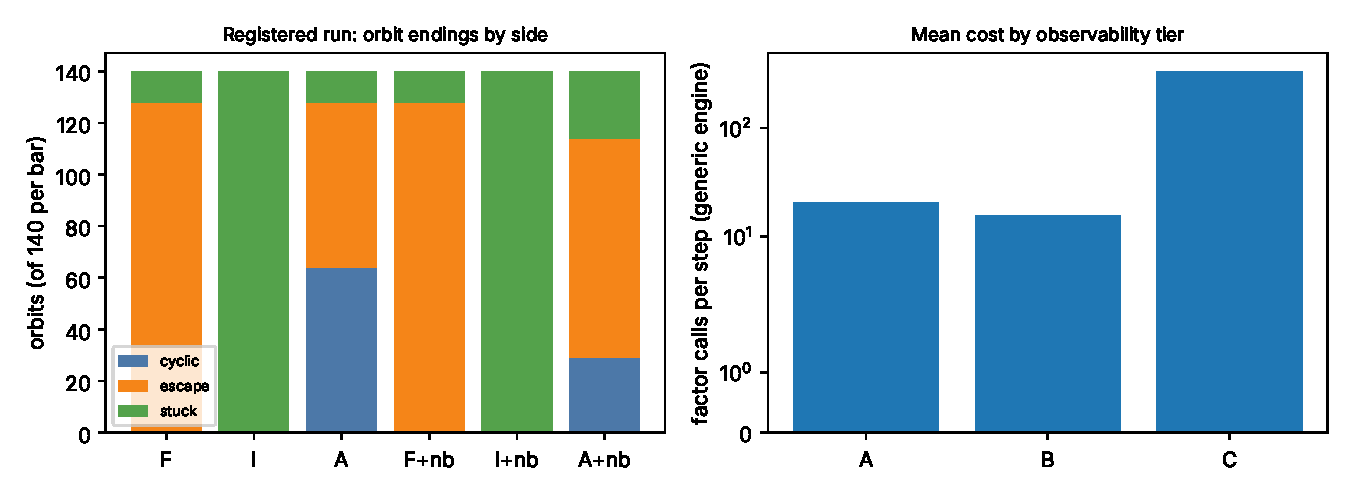
\includegraphics[width=.92\textwidth]{../figures/rn_summary.pdf}\end{center}
\textbf{Registered observations.} (a) Every orbit of the rules covered by Theorem~\ref{thm:dyn} equals its closed form (Verified-bounded above). (b) All inverse-side rules end stuck and all forward-side rules escape or are stuck at the start: N1--N3. (c) Smallest-overall without no-backtrack: all 14 orbits are 2-cycles $\{s,4s\}$ (Thm.~\ref{thm:dyn}(5)). With no-backtrack it is not stationary: it gave cycles of period 21 (e.g.\ $5,20,80,15,60,240,45,10,40,160,30,120,480,90,20,5,36,8,2,9,\dots$) and stuck orbits; this is observed, not proved. (d) Degree-min over all neighbours, without no-backtrack, gave 2-cycles for all 28 orbits; with no-backtrack and ties to the smaller value it gave 2 cyclic, 8 escaping and 4 stuck orbits. From $x_0=2$ it visits $2,9,36,5,20,125,500,45,10,121,\dots$ and reaches the primes $5,31,6763,30501131$ before leaving the bound; from $x_0=6$ it visits six distinct primes $2,5,13,31,6763,30501131$. These primes are not the next-prime sequence and no law is claimed. All orbits stay below $10^{18}$ and are certified.

\paragraph{Prior art.} The map $x\mapsto(x+1)^2$ is OEIS A004019 (Sloane; asymptotics $\lfloor c^{2^n}\rceil$ via Aho--Sloane). One web search found no source defining this graph; this is not a prior-art review, and no priority is claimed.

\paragraph{Exploratory.} Following $\sigma$ to the squarefree attractor from $x_0\le200{,}000$, the attractor is prime for a fraction \FracMinAll{} of starts (largest-inverse descent: \FracMaxI{}). No interpretation is offered.

\section{RN-3: observability and cost ledger}
Observation channels: \textbf{A} only the vertex $x$ (closed form without factoring: largest and smallest forward, i.e.\ top-1 on $F$/$A$, bottom-1 on $F$); \textbf{B} the factorization of $x$ (smallest prime factor or square part: 2nd-largest/smallest forward, top-1 and bottom-1 inverse, bottom-1 on $A$); \textbf{C} the complete neighbour set, and for degree rules the factorization of every candidate neighbour (composed from the pieces, not refactored). Counts are measured in \emph{this} Python implementation with caches cleared per orbit, three starts $\times60$ steps; ``cf'' is the closed-form evaluator of Theorem~\ref{thm:rank} where one exists.
\begin{center}\scriptsize\begin{tabular}{lcrrr}\toprule selector (no-backtrack off) & tier & factor calls/step & $\rho$ iterations/step & cf calls/step\\\midrule
F top-1 & A & 24.2 & 390.8 & 0.0\\
F top-2 & B & 22.9 & 240.6 & 1.0\\
F top-3 & C & 43.5 & 724.7 & --\\
F bottom-1 & A & 13.5 & 778.4 & 0.0\\
F bottom-2 & B & 16.1 & 1002.5 & 1.0\\
F bottom-3 & C & 39.5 & 1628.0 & --\\
F degmin/hi & C & 9.0 & 428.9 & --\\
F degmin/lo & C & 8.7 & 1315.7 & --\\
F degmax/hi & C & 2197.8 & 44230.6 & --\\
F degmax/lo & C & 1125.0 & 13233.8 & --\\
I top-1 & B & 12.0 & 0.0 & 1.6\\
I top-2 & C & 32.0 & 0.0 & --\\
I top-3 & C & 30.5 & 0.0 & --\\
I bottom-1 & B & 12.4 & 0.0 & 1.6\\
I bottom-2 & C & 32.0 & 0.0 & --\\
I bottom-3 & C & 29.5 & 0.0 & --\\
I degmin/hi & C & 12.4 & 0.0 & --\\
I degmin/lo & C & 12.4 & 0.0 & --\\
I degmax/hi & C & 13.0 & 0.0 & --\\
I degmax/lo & C & 13.0 & 0.0 & --\\
A top-1 & A & 24.2 & 390.8 & 0.0\\
A top-2 & B & 22.9 & 240.6 & 1.0\\
A top-3 & C & 43.5 & 724.7 & --\\
A bottom-1 & B & 7.2 & 0.0 & 1.0\\
A bottom-2 & C & 10.1 & 0.0 & --\\
A bottom-3 & C & 10.1 & 0.0 & --\\
A degmin/hi & C & 8.4 & 0.0 & --\\
A degmin/lo & C & 7.2 & 0.0 & --\\
A degmax/hi & C & 2197.8 & 44230.6 & --\\
A degmax/lo & C & 1125.0 & 13233.8 & --\\
\\\bottomrule\end{tabular}\end{center}
Reading: a rule can be tier A as mathematics while the generic neighbour-enumerating engine still pays tier C prices (the table shows 24 factor calls per step for the largest-neighbour rule against 0 for its closed form). Degree-max rules are the most expensive, since each candidate must be factored. These are operation counts, not intrinsic complexity.

\section{Findings and limits}
\begin{center}\small\begin{tabular}{p{.19\textwidth}p{.74\textwidth}}\toprule
\textbf{Proved} & Thm.~\ref{thm:rank}, Lemma~\ref{lem:prime}, Cor.~\ref{cor:dm}, Thm.~\ref{thm:dyn}, Cor.~\ref{cor:one}, N1--N5. All elementary; (largest neighbour) and the degree--prime equivalence are known from TI-DYN v001.\\
\textbf{Verified-bounded} & the ranges in RN-0/RN-1; \ProvedCmp{} proved-law orbit comparisons.\\
\textbf{Registered obs.} & Table of $\Orbits$ orbits; items (a)--(d).\\
\textbf{Exploratory} & terminal-prime fractions; the prime-rich degree-min orbits.\\
\textbf{Open} & dynamics of 2nd-smallest forward; periods under no-backtrack; whether any graph-local rule visits infinitely many distinct primes.\\
\textbf{Prior art} & A004019 only; no priority claimed.\\\bottomrule\end{tabular}\end{center}
\textbf{Amendments / disclosures.} None to the registration. Two notes: \texttt{rn\_closed.orbit} (registered, unused) can miss a cycle shorter than four terms, so the verifier uses its own orbit loop with the same closed-form maps; the float exponent in the small-prime sieve is disclosed in RN-0. \textbf{Unverified:} behaviour beyond horizon 400 or $10^{18}$; rank $k\ge3$ dynamics; any rule outside GL-2; whether richer observation (e.g.\ neighbours of neighbours) changes the prime picture.

\textbf{Consequence.} The graph exposes primality exactly (degree 2) but only in the two vertex families adjacent to a prime. Graph-local ranked selectors reproduce elementary dynamics (doubly exponential growth, geometric growth, finite descent, a 2-cycle) and cannot, by Corollary~\ref{cor:one}, generate primes. Degree-reading selectors are the only observed route to several primes per orbit; whether that scales is open. Recognizing a prime vertex is a theorem; generating the primes is not shown.
\end{document}
